\documentclass[12pt,a4paper]{book}
\usepackage[utf8]{inputenc}
\usepackage[portuguese]{babel}
\usepackage[T1]{fontenc}
\usepackage{amsmath}
\usepackage{amsfonts}
\usepackage{amssymb}
\usepackage{graphicx}
\usepackage{enumitem}
\usepackage{tikz}
\usetikzlibrary{matrix}

\newtheorem{example}{Exemplo}
\newtheorem{remark}{Observação}

\usepackage[left=3cm,right=2cm,top=3cm,bottom=2cm]{geometry}
\title{Matemática Aplicada e Computacional}
\author{Eduardo José de Oliveira}

\newcount\total
\newcount\lasttotal
\newcount\targetbase

\def\basetenconversiontable#1#2{%
    \begin{tikzpicture}[every node/.style={minimum width=1cm, minimum height=0.5cm}, x=1cm,y=0.5cm]
    %
    \total=#1%
    \targetbase=#2
    \def\newnumber{}
    %
    \pgfmathloop
    \ifnum\total<1
    \else
        %
        \ifnum\pgfmathcounter>1
            \node at (\pgfmathcounter, -\pgfmathcounter+1) (tmp) {\the\targetbase};
            \draw (tmp.north west) |- (tmp.south east);
            %
            %\node at (\pgfmathcounter-1, -\pgfmathcounter) (tmp) {\pgfmathparse{int(\total*\targetbase)}\pgfmathresult};
            %\draw (tmp.south west) -- (tmp.south east);
            %
            \pgfmathparse{int(\lasttotal-\total*\targetbase)}%
            \let\digit=\pgfmathresult
            \node at (\pgfmathcounter-1, -\pgfmathcounter) [text=red] {\digit};
            \edef\newnumber{\digit\newnumber}
        \fi
        %
        \ifnum\total<\targetbase
                \edef\newnumber{\the\total\newnumber}
            \node at (\pgfmathcounter, -\pgfmathcounter) [text=red]  {\the\total};
        \else
            \node at (\pgfmathcounter, -\pgfmathcounter) {\the\total};
        \fi
        \lasttotal=\total
        \divide\total by\targetbase
    \repeatpgfmathloop    
    \draw [->] (\pgfmathcounter-1,-\pgfmathcounter) -- ++(-0.5,0); 
    %\node [anchor=west] at (1, -\pgfmathcounter-2) {$#1=\newnumber_{\the\targetbase}$};
    \end{tikzpicture}   
}

\def\basetenconversiontabledemo{
	\begin{tikzpicture}[every node/.style={minimum width=1cm, minimum height=0.5cm}, x=1cm, y=0.5cm]
		\node at (1, -1) {$N$};
	
		\node at (2, -1) (tmp) {2};
		\draw (tmp.north west) |- (tmp.south east);
		\node at (1, -2) [text=red] {$r_1$};

		\node at (2, -2) {$q_1$};
		
		\node at (3, -2) (tmp) {2};
		\draw (tmp.north west) |- (tmp.south east);
		\node at (2, -3) [text=red] {$r_2$};
		\node at (3, -3) {$q_2$};
		
		\node at (4, -3) (tmp) {2};
		\draw (tmp.north west) |- (tmp.south east);
		\node at (3, -4) [text=red] {$r_3$};
		\node at (4, -4) {$q_3$};
		
		\node at (5, -5) {$\ddots$};
		\node at (6, -6) {$q_{n-1}$};
		\node at (7, -6) (tmp) {2};
		\draw (tmp.north west) |- (tmp.south east);
		\node at (6, -7) [text=red] {$r_n$};
		\node at (7, -7) [text=red] {1};
		
		\draw [->] (7, -8) -- ++(-1,0);
		\draw [->] (6, -8) -- (1, -3);
	\end{tikzpicture}
}

\newenvironment{tablePontoFlutuante16bits}{
	\begin{figure}[h]
		\centering
		\begin{tikzpicture}
			\matrix (num_rep) [matrix of nodes] 
}{
			\draw (num_rep-1-1.north west) rectangle (num_rep-1-16.south east);
			\foreach \i in {1,...,16}{
				\draw (num_rep-1-\i.north west) -- (num_rep-1-\i.south west);
			}
		\end{tikzpicture}
	\end{figure}
}

\newcommand{\todo}[1]{
	{\color{red}#1}
}

\begin{document}


%
%
%
\chapter{Introdução}

As fases na resolução de problemas em matemática aplicada e computacional que surgem nas mais diversas áreas do conhecimento, de modo geral, podem ser representadas da seguinte maneira:

\begin{figure}[h]
	\centering
	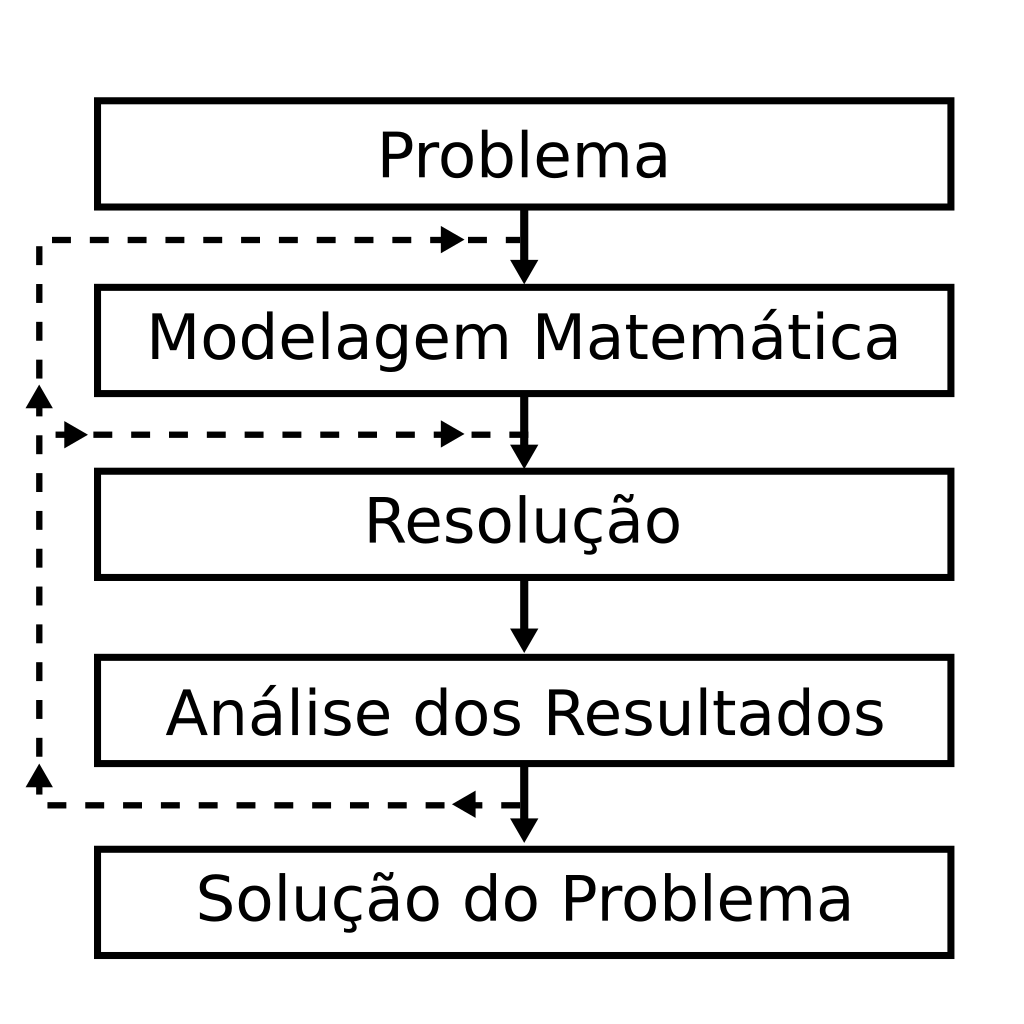
\includegraphics[scale=0.2]{figuras/figura_001}
	\caption{Fluxograma das fases na resolução de problemas em Matemática Aplicada e Computacional.}
\end{figure}

A primeira fase consiste basicamente em definir corretamente o problema a ser solucionado. A fase da modelagem matemática é onde ocorre a construção ou definição do modelo matemático que irá descrever o comportamento do problema em questão. Na fase de resolução são definidos e implementados os métodos para obtenção da solução do problema.

A análise dos resultados tem por finalidade verificar os resultados obtidos na resolução do problema. Se o resultado for satisfatório aceitamos a solução do problema, caso contrário, deve-se procurar outros métodos ou refazer a modelagem matemática.

%
%
%
\chapter{Principais erros na resolução de um problema}

Na resolução de um problema os erros podem surgir em cada fase. A seguir apresentamos os principais:

\section{Erros na fase do problema}

Não definir corretamente o problema é um erro grave que pode levar a falsos resultados.

\section{Erros na modelagem matemática}

O modelo matemático para um problema real deve representar o fenômeno que ocorre no mundo físico, porém, nem sempre é fácil. Normalmente são necessárias simplificações no modelo físico para se obter um modelo matemático (tratável) que fornecerá uma solução para o problema. Essas simplificações se constituem em fonte de erros, o que pode acarretar na necessidade de reformular o modelo matemático adotado.

\begin{example}
	Um matemático quer determinar a altura de um edificio dispondo de uma esfera de metal, um cronômetro e a equação $s=s_0+v_0 t+ \frac{1}{2}at^2$. Para isso, ele sobe no topo do edificio e solta a esfera de metal anotando o tempo até a mesma tocar o solo, ou seja, 3 segundos.
	
	\begin{figure}[h]
		\centering
		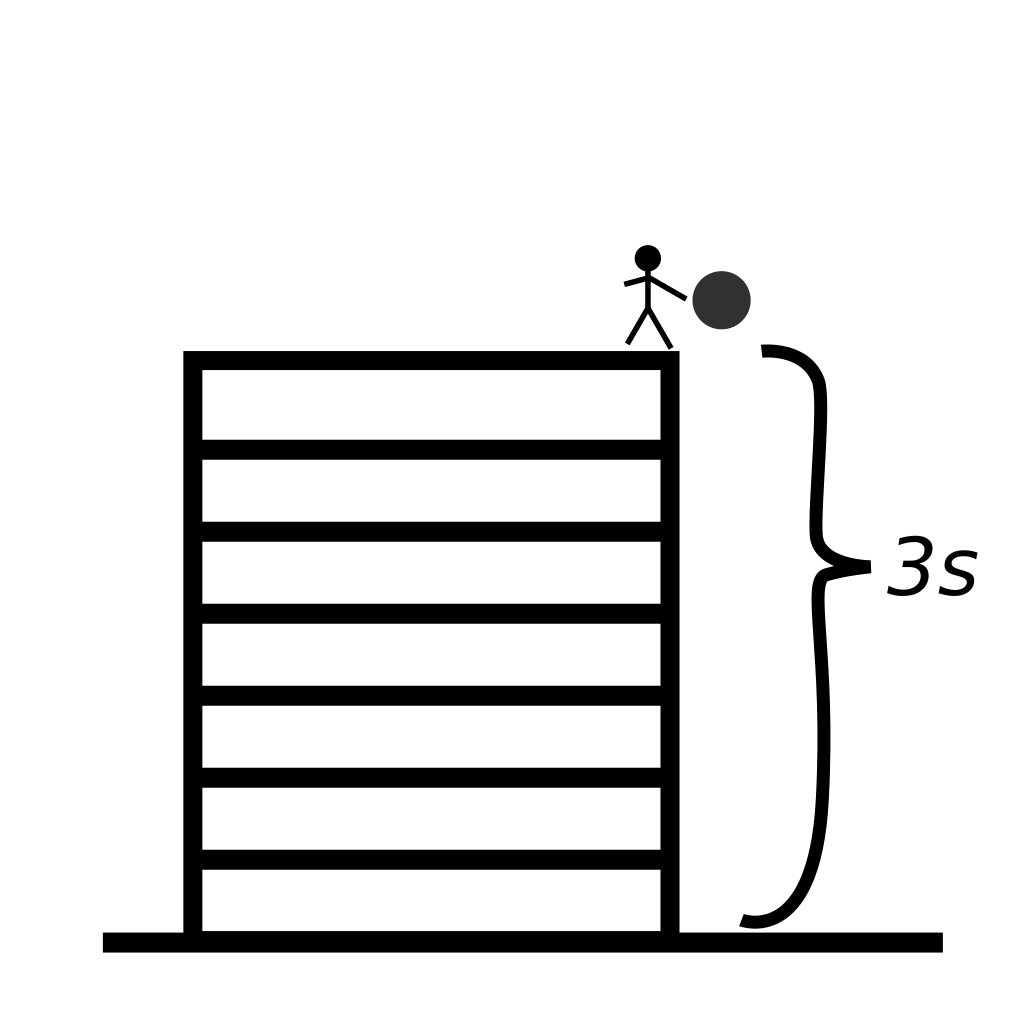
\includegraphics[scale=0.15]{figuras/figura_002}
	\end{figure}
	
	Logo, tem-se $s=s_0+v_0 t+\frac{1}{2}at^2=0+0\cdot 3 + \frac{1}{2}\cdot 9,8 \cdot 3^2=44,1$ m.
	
	Esse resultado é confiável?
	
	Provavelmente não, pois o modelo matemático utilizado não considera outras variáveis relevantes como, por exemplo, a resistência do ar, a velocidade do vento dentre outras.
	
	Além disso, há outro fato que pode influenciar diretamente a precisão na leitura do cronômetro, pois uma pequena variação nessa leitura pode acarretar uma grande variação no cálculo da altura do edificio. Se o tempo medido fosse de 3,5 segundos ao invés de 3 segundos, a altura do edificio seria calculada em 60,025 m. Ou seja, uma variação de 16,67\% na leitura do cronômetro ocasiona uma variação de 36,11\% no cálculo da altura do edifício.
	
	Logo pode-se notar a influência que o modelo matemático e a precisão dos dados de entrada exercem sobre a confiabilidade dos resultados.
\end{example}

\begin{remark}
	Durante a aula, foi proposta uma atividade semelhante em que, utilizando o cronômetro dos celulares e uma bolinha, em duplas, realizando procedimento parecido com o do exemplo, os alunos deveriam estimar a altura da porta da sala de aula.
\end{remark}

\section{Erros na resolução}

Esses erros podem ocorrer na representação de números, na conversão da base e também nos arredondamentos.

Na representação de números, considere o cálculo da área de uma circunferência de raio 100 m, onde utilizaremos os seguintes valores para $\pi$:
\begin{enumerate}[label=\Alph*]
	\item $\pi=3,14\Longrightarrow A=31.400 m^2$.
	\item $\pi=3,1416\Longrightarrow A=31.416 m^2$.
	\item $\pi=3,141592654\Longrightarrow A=31.415,93 m^2$.
\end{enumerate}

A representação de um número depende da base escolhida ou disponível na maquina em uso (computador, calculadora) e do número máximo de dígitos usados na sua representação.

O número $\pi$ não pode ser representado, através de um número finito de dígitos decimais. Neste exemplo utilizou-se três valores para $\pi$, sendo que para cada valor foi encontrado um resultado diferente para a área da circunferência. O erro neste exemplo depende exclusivamente da aproximação escolhida para $\pi$. Qualquer que seja a circunferência, a sua área nunca será obtida exatamente, uma vez que $\pi$ é um número irracional.

Qualquer cálculo que envolva números que não podem ser representados através de um número finito de dígitos não fornecerá como resultado um valor exato. Quanto maior o número de dígitos utilizados, maior será a precisão obtida. Por isso, a melhor aproximação, neste exemplo, para o valor da área da circunferência é quando $\pi=3,141592654$ (caso (c)).

Na conversão de base pode ocorrer que um número tenha representação finita em uma base e não finita em outra base. Por exemplo, o número 0,6 na base decimal é representado pelo número 0,10011001$\dots$ na base 2, isto é:
$$
	(0,6)_{10}=(0,10011001\dots)_{2}
$$

É usual representar e realizar operações com números na base 10 (decimal), mas um número real pode ser representado em qualquer base. Um computador, normalmente, opera no sistema binário, ou seja, base 2.

Em relação ao arredondamento, observe que na interação entre usuário e o computador que opera na base binária, ocorre o seguinte: os dados de entrada são enviados ao computador pelo usuário no sistema decimal e toda essa informação é convertida para a base binária pelo computador e as operações são efetuadas nessa base. Os resultados obtidos no sistema binário são convertidos para o sistema decimal e transmitidos ao usuário.

Todo esse processo de conversão de base pode se constituir em uma fonte de erros de arredondamentos que pode afetar os resultados finais dos cálculos na resolução de um problema.

\begin{example}
	Considere os seguintes valores $x_1=0,003815$ e $x_2=1.234.567.890$ e, as operações $(x_1+x_2)-x_2$ e $x_1+(x_2-x_2)$. Temos os seguintes resultados:

	\begin{itemize}
		\item \textbf{Calculadora científica (10 digitos):}\hfill
		$$(x_1+x_2)-x_2=(0,003815+1.234.567.890)-1.234.567.890=$$
		$$=1.234.567.890-1.234.567.890=0\text{,}$$
		e, no segundo caso,
		$$x_1+(x_2-x_2)=0,003815+(1.234.567.890-1.234.567.890)=$$
		$$=0,003815+0=0,003815\text{.}$$
	\end{itemize}
	\todo{Complementar o exemplo falando sobre o uso de cálculadoras de celular, linguagens de programação (tamanho máximo de números), etc.}
\end{example}

\chapter{Representação de Números}

Em geral, um número real $x$ na base $\beta$ é representado por
$$
	x=(a_{m}a_{m-1}\cdots a_2 a_1 a_0, b_1 b_2\cdots b_k)_{\beta}
$$
$$
	x=a_{m}\cdot \beta^{m}
	+
	a_{m-1} \cdot \beta^{m-1}
	+ \cdots +
	a_1 \cdot \beta^1
	+
	a_0 \cdot \beta^0
	+
	b_1 \cdot \beta^{-1}
	+
	b_2 \cdot \beta^{-2}
	+ \cdots +
	b_k \cdot \beta^{-k}
	\text{,}
$$
onde $0\leqslant a_i < \beta$, $i=0$, $1$, $2$, $\dots$, $m$ e $0\leqslant b_j < \beta$, $j=1$, $2$, $\dots$, $k$.

De fato, no sistema decimal temos que $\beta=10$ e $a_i$ e $b_j$ elementos do conjunto $A=\{$0, 1, 2, 3, 4, 5, 6, 7, 8, 9$\}$, no binário temos que $\beta=2$ e $a_i$ e $b_j$ são elementos do conjunto $A=\{$0, 1$\}$.

\begin{example}
	Escreva a representação dos seguintes números:
	\begin{enumerate}
  		% exemplo 1
	    \item $x=(1984)_{10}$ = $1\cdot 10^3 + 9\cdot 10^2 + 8\cdot 10^1 + 4\cdot 10^0$.
    	% exemplo 2
	    \item $x=(15,47)_{10}$ = $1\cdot 10^1 + 5\cdot 10^0 + 4\cdot 10^{-1} + 7\cdot 10^{-2}$.
	    % exemplo 3
    	\item $x=(0,362)_{10}$ = $0\cdot 10^0 + 3\cdot 10^{-1} + 6\cdot 10^{-2} + 2\cdot 10^{-3}$.
	    % exemplo 4
    	\item $x=(1011)_{2}$ = $1\cdot 2^3 + 0\cdot 2^2 + 1 \cdot 2^1 + 1 \cdot 2^0$.
	    % exemplo 5
    	\item $x=(11,01)_{2}$ = $1\cdot 2^1 + 1\cdot 2^0 + 0\cdot 2^{-1} + 1\cdot 2^{-2}$.
	    % exemplo 6
    	\item $x=(0,110)_{2}$ = $0\cdot 2^0 + 1\cdot 2^{-1} + 1\cdot 2^{-2} + 0\cdot 2^{-3}$.
	    % exemplo 7
    	\item $x=(1572)_{8}$ = $1\cdot 8^3 + 5\cdot 8^2 + 7\cdot 8^1 + 2\cdot 8^0$.
	    % exemplo 8
    	\item $x=(0,1)_{4}$ = $0\cdot 4^0 + 1 \cdot 4^{-1}$.
	\end{enumerate}
\end{example}

\section{Conversão de Bases}

\subsection{Binário para Decimal}

Para converter da base binária para a base decimal, basta multiplicar o dígito binário por uma potência $\beta=2$ adequada, ou seja, resolver a expressão da representação numérica na base decimal.

\begin{example}
    Converta os seguintes números para a base decimal:
    \begin{enumerate}
        % exemplo a
        \item $(101101)_{2}$ = $1\cdot 2^5 + 0\cdot 2^4 + 1 \cdot 2^3 + 1 \cdot 2^2 + 0\cdot 2^1 + 1\cdot 2^0$, ou seja, $(101101)_{2} = 32 + 0 + 8 + 4 + 0 + 1 = 45$. Portanto, $(101101)_{2}=(45)_{10}$.
        % exemplo b
        \item $(1011,110)_{2}$ = $1\cdot 2^3 + 0 \cdot 2^2 + 1 \cdot 2^1 + 1 \cdot 2^0 + 1 \cdot 2^{-1} + 1\cdot 2^{-2} + 0 \cdot 2^{-3}$, donde $(1011,110)_{2}=(11,75)_{10}$.
        % exemplo c
        \item $(1251)_{8}$ = $1\cdot 8^3 + 2 \cdot 8^2 + 5\cdot 8^1 + 1\cdot 8^0 = (681)_{10}$.
        % exemplo d
        \item $(0,1)_{4}$ = $0\cdot 4^0 + 1 \cdot 4^{-1}=(0,25)_{10}$.
    \end{enumerate}
\end{example}

\subsection{Decimal para Binário}

Para a conversão de um número na base 10 para a base 2, utiliza-se um processo para a parte inteira e um outro diferente para a parte fracionária.

Para converter a parte inteira, utiliza-se o processo das divisões sucessivas, que consiste em dividir a parte inteira do número por 2. A seguir, divide-se por 2 o quociente encontrado e assim o processo é repetido até que o último quociente seja igual a 1. 

O número binário será formado pela concatenação dos restos das divisões lidos em sentido inverso a que foram obtidos com o número 1 (último quociente) sendo o primeiro digito desse número, isto é:

\begin{figure}[h]
	\centering
	\basetenconversiontabledemo
\end{figure}

Logo, tem-se que $(N)_{10}=(1r_n r_{n-1}\cdots r_3 r_2 r_1)$.

\begin{example}
	Converta os seguintes números para binário
	\begin{enumerate}
	    \item $(17)_{10}$.\hfill
	    	\begin{figure}[h]
	    		\centering
		    	\basetenconversiontable{17}{2}
	    	\end{figure}
	    	
	    	Logo, $(17)_{10}=(10001)_{2}$.
	    	\newpage
	    	
	    \item $(26)_{10}$.\hfill
	    	\begin{figure}[h]
	    		\centering
	    		\basetenconversiontable{26}{2}
	    	\end{figure}
	    	
	    	Logo, $(26)_{10}=(11010)_{2}$.
    	\item $(100)_{10}$.\hfill
    		\begin{figure}[h]
    			\centering
    			\basetenconversiontable{100}{2}
    		\end{figure}
    		
    		Logo, $(100)_{10}=(1100100)_{2}$.
	\end{enumerate}
\end{example}

Para converter a parte fracionária de um número na base 10 para a base 2, utiliza-se o processo das multiplicações sucessivas. Multiplica-se a parte fracionária por 2, deste resultado, a parte inteira será o primeiro dígito (após a vírgula) do número binário e a parte fracionária será novamente multiplicada por 2. Desse resultado, a parte inteira será o segundo dígito do número binário e a parte fracionada será multiplicada novamente por 2. Repete-se esse processo até que a parte fracionada do último produto seja igual a zero, no caso do número ter representação finita.

\begin{example}
    Converta os números a seguir para a base binária.
    \begin{enumerate}
        \item $(0,125)_{10}$. Como $0,125\cdot 2 = 0,25$, o primeiro dígito é 0. Ainda, $0,25\cdot 2=0,5$, logo, o segundo dígito é 0. $0,5\cdot 2=1$, donde o terceiro dígito é $1$. Logo, $(0,125)_{10}=(0,001)_{2}$.
        
        \item $(0,185)_{10}$. Como $0,185\cdot 2=0,37$, o primeiro dígito é 0. Ainda, $0,37\cdot 2=0,74$, o segundo dígito é 0. $0,74\cdot 2=1,48$, donde o terceiro dígito é 1. $0,48\cdot 2=0,96$, donde o quarto dígito é 0. $0,96\cdot 2=1,92$, onde o quinto dígito é 1. $0,92\cdot 2=1,84$, donde o sexto dígito é $1$. $0,84\cdot 2=1,68$, então o setimo dígito é 1. Como a parte fracionária irá sempre se reptir, sua representação binária é infinita, então $(0,185)_{10}=(0010111\dots)_{2}$.

        \item $(13,25)_{10}$ \todo{fazer a resolução}

        \item $(3,8)_{10}$ \todo{fazer a resolução}
    \end{enumerate}
\end{example}

\section{Aritmética de Ponto Flutuante}

As maquinas, cmo computadores e calculadoras, utilizam uma quantidade fixa de dígitos para representar um número real no sistema denominado de aritmética de ponto flutuante. Um número real na base $\beta$ em aritmética de ponto flutuante de $t$ dígitos, tem forma geral
$$
    \pm
    0.d_{1}d_{2}d_{3}\cdots d_{t}\cdot \beta ^{e}
    \text{,}
$$
onde $0 \leqslant d_i < \beta$, $i=1$, 2, $\dots$, $t$. Ainda, $t$ é o número de dígitos significativos, $\beta$ é a base em que a maquina opera e $e$ é o expoente no intervalo $[m, M]$, com $m$ e $M \in \mathbb{Z}$. $d_1$, $d_2$, $d_3$, $\dots$, $d_t$ são chamados de mantissa.

Em geral, $m=-M$. Se $d_1\neq 0$, caracteriza o sistema em ponto finalmente normalizado.

\begin{example}
    Represente os números a seguir num sistema de aritmética de ponto flutuante (normalizado).
    \begin{enumerate}
    	\item $(5720)_{10}$ = $0.5720\cdot 10^4$.
	    \item $(90621)_{10}$ = $0.90621\cdot 10^5$.
    	\item $(51,734)_{10}$ = $0.51734\cdot 10^2$.
	    \item $(0,00913)_{10}$ = $0.913\cdot 10^{-2}$.
    	\item $(-0,0001)_{10}$ = $-0.1\cdot 10^{-3}$.
	    \item $(101101)_{2}$ = $0.101101\cdot 2^{6}$ e, transformando 6 em binário, tem-se $0.101101\cdot 2^{110}$.
    	\item $(110,101)_{2}$ = $0.110101\cdot 2^3$ e, transformando 3 em binário, tem-se $0.110101\cdot 2^{11}$.
	    \item $(0,01101)_{2}$ = $0.1101\cdot 2^{-1}$.
    	\item $(-0,0001001)_{2}$ = $-0.1001\cdot 2^{-3}$ e, convertendo 3 para a base binária, tem-se $-0.1001\cdot 2^{-11}$.
	\end{enumerate}
\end{example}

Um número não poderá ser representado na maquina com sistema de aritmética do ponto flutuante se o expoente $e$ estiver fora do intervalo $[m, M]$. A maquina acusará o erro de \textit{underflow} se $e < m$ e de \textit{overflow} se $e>M$.

\begin{example}
    Considere uma maquina que opera no sistema de aritmetica de ponto flutuante com $\beta=10$, $t=3$ e $e\in [-2, 2]$. Represente neste sistema os seguintes números decimais.
    \begin{enumerate}
        \item $0,35 = 0.350\cdot 10^0$
        \item $-5,172 = -0.517\cdot 10^1$
        \item $0,0123 = 0.123\cdot 10^{-1}$
        \item $5391,3 = 0.539\cdot 10^4$, como 4 não está no intervalo entre -2 e 2, $4 > 2$, a maquina acusará o erro de overflow.
        \item $0,0003 = 0.3\cdot 10^{-3}$, como 3 não está no intervalo entre -2 e 2, $-3 < -2$, a maquina acusará o erro de underflow.
    \end{enumerate}
\end{example}

\begin{remark}
	Algumas linguagens computacionais permitem trabalhar em precisão dupla, que é o mesmo sistema de aritmética de ponto flutuante, mas com o dobro de dígitos disponíveis na mantissa. Vale lembrar que nesse caso, o tempo de execução e a memória usada aumentam significativamente.
\end{remark}

Para representar um sistema de ponto flutuante normalizado na base $\beta$, com $t$ dígitos significativos e expoente $e \in [m, M]$, usaremos a seguinte notação:
$$F(\beta, t, m, M)\text{.}$$

\begin{example}
    Dado o sistema de aritmética de ponto flutuante $F(10, 3, -4, 4)$, represente os seguintes números decimais nesse sistema:
    \begin{enumerate}
        \item $1,35$ = $0.135\cdot 10^1$.
        \item $-279,15$ = $-0.279\cdot 10^3$.
        \item $0,024712$ = $0.247\cdot 10^{-1}$.
        \item $10,13$ = $0.101\cdot 10^2$.
    \end{enumerate}
\end{example}

\begin{example}
    Dado $F(2, 10, -15, 15)$ represente os seguintes números nesse sistema de aritmética de ponto flutuante:
    \begin{enumerate}
        \item $(11001)_2 = 0.1100100000\cdot 2^{101}$.
        \item $(45)_{10} = (101101)_2 = 0.1011010000\cdot 2^{110}$.
        \item $(-7,125)_{10} = (-111,001)_2 = -0.1110010000\cdot 2^{-11}$.
    \end{enumerate}
\end{example}

\begin{example}
    Considere o sistema $F(2, 3, -1, 2)$. Quantos e quais números podem ser representados neste sistema?

    São os números $\pm 0.100\cdot 2^e$, $\pm 0.110\cdot 2^e$, $\pm 0.101\cdot 2^e$, $\pm 0.111 \cdot 2^e$, onde $e \in [-1, 2]$. Como temos 4 possibilidades para $e$, são 32 números nesse formato, extendendo ao zero, 33.
\end{example}

\begin{remark}
    Sabemos que os números reais podem ser representados por uma reta contínua. Entretanto, em ponto flutuante podemos representar apenas pontos discretos na reta real.
\end{remark}

\begin{example}
    Considerando, ainda, o sistema do exemplo anterior $F(2, 3, -1, 2)$, represente os seguintes números:
    \begin{enumerate}
        \item $(0,38)_{10} = (0,0110110\dots)_2=0.110\cdot 2^{-1}$.
        \item $(0,375)_{10} = (0.110)_2 = 0.110\cdot 2^{-1}$.
        \item $(5,3)_{10} = (101,01001\dots)_2 = 0.101\cdot 2^{11}$. Mas como o expoente é limitado entre -1 e 2 (decimais), o número seria um caso de overflow.
    \end{enumerate}
\end{example}

\subsection{Representação de um número na máquina}

Um número é representado, internamente, numa máquina digital através de uma sequência de impulsos elétricos que indicam dois estados: 0 ou 1, ou seja, na base binária. Cada dígito é chamado de bit. Suponha uma máquina que utiliza 16 bits da seguinte maneira:
\begin{itemize}
    \item 10 bits para representar a mantissa;
    \item 4 bits para representar o expoente;
    \item 1 bit para representar o sinal da mantissa;
    \item 1 bit para representar o sinal do expoente.
\end{itemize}

Para representar o sinal, utiliza-se:
\begin{itemize}
    \item Para o sinal positivo utiliza-se o bit 0;
    \item para o sinal negativo, utiliza-se o bit 1.
\end{itemize}

Observando a representação na tabela a seguir, o local marcado como 1 representa o sinal da mantissa. Os lugares marcados de 2 a 11 representam a mantissa. O lugar marcado como 12 representa o sinal do expoente enquanto os lugares marcados de 13 a 16 representam o expoente.
\begin{figure}[h]
	\centering
	\begin{tikzpicture}
		\matrix (num_rep) [matrix of nodes] {
			|[fill=green!30]|1 & |[fill=blue!30]|2 & |[fill=blue!30]|3 & |[fill=blue!30]|4 & |[fill=blue!30]|5 & |[fill=blue!30]|6 & |[fill=blue!30]|7 & |[fill=blue!30]|8 & |[fill=blue!30]|9 & |[fill=blue!30]|10 & |[fill=blue!30]|11 & |[fill=green!30]|12 & |[fill=red!30]|13 & |[fill=red!30]|14 & |[fill=red!30]|15 & |[fill=red!30]|16   \\
		};
		\draw (num_rep-1-1.north west) rectangle (num_rep-1-16.south east);
		\foreach \i in {1,...,16}{
			\draw (num_rep-1-\i.north west) -- (num_rep-1-\i.south west);
		}
	\end{tikzpicture}
\end{figure}

\begin{example}
	\begin{enumerate}
		\item O número $(25)_{10} = (11001)_2 = 0.11001\cdot 2^{101}$ pode ser representado como:
		\begin{tablePontoFlutuante16bits}
			{
			0 & 1 & 1 & 0 & 0 & 1 & 0 & 0 & 0 & 0 & 0 & 0 & 0 & 1 & 0 & 1 \\
			};
		\end{tablePontoFlutuante16bits}
		
		\item O número $(-7,125)_{10}=(-111,001)_2 = -0.111001\cdot 2^{11}$ pode ser representado como:
		\begin{tablePontoFlutuante16bits}
			{
			1 & 1 & 1 & 1 & 0 & 0 & 1 & 0 & 0 & 0 & 0 & 0 & 0 & 0 & 1 & 1 \\
			};
		\end{tablePontoFlutuante16bits}
		\newpage
		\item O número $(0,1)_{10}=(0,000110011\dots)_2 = 0.1100110011\cdot 2^{-11}$ pode ser representado como:
		\begin{tablePontoFlutuante16bits}
			{
			0 & 1 & 1 & 0 & 0 & 1 & 1 & 0 & 0 & 1 & 1 & 1 & 0 & 0 & 1 & 1 \\
			};
		\end{tablePontoFlutuante16bits}
	\end{enumerate}
\end{example}

\subsection{Truncamento e Arredondamento}

Seja $x$ um número decimal na forma $0.d_1 d_2 \dots d_t d_{t+1} \dots \cdot \beta ^e$. Para truncar ou arredondar esse número $x$ para um número $\overline{x}$ com $t$ casas decimais utiliza-se os seguintes procedimentos:
\begin{itemize}
    \item No truncamento despreza-se todos os dígitos após a $t$-ésima casa decimal ou após o dígito $d_t$, isto é: $\overline{x}=0.d_1 d_2 \dots d_t \cdot \beta^e$.

    \item No arredondamento, se o dígito $d_{t+1}$ é menor que 5 despreza-se todos os dígitos posteriores a $d_t$ (truncamento). Porém, se $d_{t+1}$ é maior ou igual a 5 soma-se 1 ao dígitos $d_t$ e despreza-se os dígitos posteriores a ele.
\end{itemize}

\begin{example}
    Utilizando truncamento e arredondamento passe os números a seguir para 4 casas decimais:

    \begin{enumerate}
        \item $x=0.77712345\cdot 10^3$.
        	\begin{itemize}
			    \item Truncamento: $\overline{x}=0.7771\cdot 10^3$.
			    \item Arredondamento: $\overline{x}=0.7771\cdot 10^3$.
			\end{itemize}

        \item $y=0.86537\cdot 10^{-5}$.
        	\begin{itemize}
			    \item Truncamento: $\overline{y}=0.8653\cdot 10^{-5}$.
			    \item Arredondamento: $\overline{y}=0.8654\cdot 10^{-5}$.
			\end{itemize}
			
    \end{enumerate}
\end{example}

\begin{example}
    Considere o sistema $F(10,3,-5,5)$. Represente os seguintes números nesse sistema utilizando truncamento e arredondamento.

    \begin{enumerate}
        \item $x=1234,56$.
	        \begin{itemize}
			    \item Truncamento: $\overline{x}=0.123\cdot 10^{4}$.
			    \item Arredondamento: $\overline{x}=0.123\cdot 10^{4}$.
			\end{itemize}

        \item $y=-0,00054962$.
        	\begin{itemize}
			    \item Truncamento: $\overline{y}=-0.549\cdot 10^{-3}$.
			    \item Arredondamento: $\overline{y}=-0.550\cdot 10^{-3}$.
			\end{itemize}

        \item $z=0,9995$.
        	\begin{itemize}
			    \item Truncamento: $\overline{z}=0.999\cdot 10^{0}$.
			    \item Arredondamento: $\overline{z}=1.000\cdot 10^{1}$.
			\end{itemize}

        \item $w=123456,7$.\\
        	$w=0.1234567\cdot 10^6$. Erro de overflow.

        \item $v=-0,0000001$.\\
        	$v=-0.1\cdot 10^{-6}$. Erro de underflow.
    \end{enumerate}
\end{example}

\section{Erro Absoluto e Relativo}

Quando se calcula um resultado por aproximação é preciso saber como estimar ou delimitar o erro cometido na aproximação. 

Em geral, apenas o valor aproximado é conhecido, e, neste caso, é impossível obter o valor exato do erro, mas pode-se estimar o erro ou até delimitá-lo obtendo-se um limite superior.

Para se estimar ou delimitar o erro, recorre-se a dois conceitos: o erro absoluto e erro relativo.

\subsection{Erro Absoluto}

É a diferença, em módulo, entre o valor exato de um número e o seu valor aproximado, isto é:
$$
    |EA_x|=|x-\overline{x}|
    \text{,}
$$
onde $x$ é o valor exato e $\overline{x}$ é o valor aproximado.

\begin{example}
    Considere o número $9,4318$ e uma máquina que opera apenas com 3 dígitos. Qual o erro absoluto cometido por essa máquina para representar esse número?

    $x=9,4318 \Longrightarrow \overline{x}=9,43$. Assim, $|EA_x|=|x-\overline{x}|$, ou seja, $|EA_x|=|9,4318-9,43|=0,0018$ ou ainda $0.180\cdot 10^{-2}$.
\end{example}

\begin{example}
    Sabendo-se que $\pi \in (3,14; 3,15)$. Determine o erro absoluto que se pode cometer ao escolher um valor desse intervalo para $\pi$.

    $|EA_{\pi}|=|\pi-\overline{\pi}|<0,01$ ou, ainda, $0.1\cdot 10^{-1}$.
\end{example}

\begin{example}
    Seja $x$ um número representado por $\overline{x}=7,3$ de tal forma que $|EA_x|<0,1$. Determine o menor intervalo que contenha $x$.

    O intervalo é dado por $(7,3-|EA_x|;7,3+|EA_x|)$ que é $(7,3-0,1;7,3+0,1)$, isto é, $(7,2;7,4)$.
\end{example}

\end{document}